\documentclass[a4paper,twocolumn,11pt]{quantumarticle}
\pdfoutput=1
\usepackage[utf8]{inputenc}
\usepackage[english]{babel}
\usepackage[T1]{fontenc}
\usepackage{amsmath}
\usepackage{hyperref}

\usepackage{tikz}
\usepackage{lipsum}

\usepackage{natbib}
\bibliographystyle{unsrt}

\newtheorem{theorem}{Theorem}
\begin{document}

\title{Solus: An end-to-end AI software developer.}

\author{Adam Blumenfeld}
\affiliation{President, CSX Labs}
\email{adamb@csxlabs.org}
\orcid{0000-0001-9995-3327}
\maketitle

\begin{abstract}
  TODO: Fill in abstract.
\end{abstract}
\section{Introduction}
\subsection{Market Background}
The seamless transfer of knowledge and data across nations powered the information age. Global access to electronic devices created high-growth platforms and services, springing millions of jobs in content creation, software development, and more. An estimated 26.9 million professional developers practiced worldwide as of 2022, growing 14.5\% from 2018\cite{Qubit2022How}. The inception of large language models gave rise to the generative AI space, with platforms growing at a record pace, such as OpenAI's ChatGPT, which rose to 100 million users in two months\cite{Carr2023ChatGPT}. One implication of generative AI is that it automates large portions of the jobs created in the information revolution in the tech, legal, financial, media, and support fields, to name a few\cite{Mok2023ChatGPT}. S\&P Global Market Intelligence predicts generative AI market revenue to hit \$36 billion by 2028, forecasting code generators to lead the expansion at a compound annual growth rate of 72.9\%\cite{Park2023Generative}. The ability of language models to generate code has sparked new products such as GitHub's Copilot\cite{Dohmke2022GitHub}, Replit's Ghostwriter\cite{Masad2022Ghostwriter}, and Amazon's Codewhisperer\cite{Engdahl2023Amazon}, which provide inline code completions saving developers time from repetitive tasks, routine lookups, and forgotten implementations.

Inline completions are helpful but far from autonomous, requiring manual developer intervention and revision.

Projects like Smol\cite{Osika2023Current}, AutoGPT\cite{Ortiz2023What}, and BabyAGI\cite{Parthasarathy2023Meet} aim to perform tasks autonomously by making language models reason and evaluate themselves. However, projects like AutoGPT and BabyAGI are general in project scope, leading to a jack-of-all-trades issue.

In contrast, Smol is simple though it lacks capability and requires much human intervention.

\subsection{Problems}
\subsubsection{Scope Limits Capability}
Tools like AutoGPT and BabyAGI aim to achieve artificial general intelligence (AGI), a system that can learn to carry out any task a human or animal can perform\cite{Bubeck2023Sparks}. Although a novel goal, refraining from tailoring the generative process to a specific task limits the value, the systems can bring to such a complex task as software development. A capable AI software developer project must tailor agents to the software development lifecycle.

\subsubsection{Multi-Agent Collaboration}
There are no effective frameworks for multi-agent communication and
collaboration on a resource in an organized manner. Software development is an
inherently complex process, with many scoped concerns spanning a project with
many dependencies and business-related tradeoffs to weigh in. As agents act on a
project's resources, a standard protocol must exist for compartmentalizing
working areas, communicating issues, and resolving conflicts.

\subsubsection{Manual Feedback Loop}
Most tools require an amount of human feedback and approval when operating to
stay on track and approve resource usage. Language model costs incurred during
critical reasoning and self-regulation limit more capable projects, such as
AutoGPT. These costs are a barrier to making multi-agent systems possible, as the
quality of these tools' performance as software developers render the cost
unjustified. Therefore, an AI software developer system must have transparent
resource monitoring and self-guidance, ensuring the quality of iteration.

\subsection{Solution}
Solus \textit{will be}\footnote{NOTE: We are raising funding to build Solus due to the steep upstart costs. Contact the corresponding author if you want to contribute financially.} an end-to-end AI software development solution utilizing self-critical, multi-role AI agents.

\subsubsection{System Requirements}
Solus must be robust, secure, and scalable to be a suitable system for enterprises to trust with their projects.

We achieve this by compartmentalizing agents and adding layers of abstraction to inter-agent communication, allowing us to optimize, shard, and secure resources under the hood.

\subsubsection{Product Requirements}
The system must be capable of doing most software development tasks, such as managing dependencies, refactoring, debugging, and generating business logic and documentation related to the project and business goals. It must execute these tasks self-regulating while ensuring all operations are transparent, traceable, and intervenable. We accomplish this by orchestrating the agents in a service mesh where sidecars intercept communications between agents and resources and beam them to a centralized control plane that controls downstream processes and provides visibility over the operation.

\subsubsection{Business Requirements}
Solus must be versatile, profitable, and sustainable. By making agents customizable components with a clear separation of concerns, we can give Solus a clear path of expansion to other applications in the generative AI space. By operating on a cloud model, we can stay profitable on a low operating margin, minimizing costs for us and our customers. To make Solus sustainable, we plan on creating a plugin ecosystem for optimized agent types for specific tasks and technologies. These developer ecosystems give Solus an economic moat over other initiatives. We also plan on building Solus to be open-source to ensure the most significant impact on the developer community. Open source allows us to create an ecosystem around our technology while maintaining profit and advantage due to enterprise trust in our platform.

\section{System Architecture}
\subsection{Components}
\begin{figure*}[t]
  \centering
  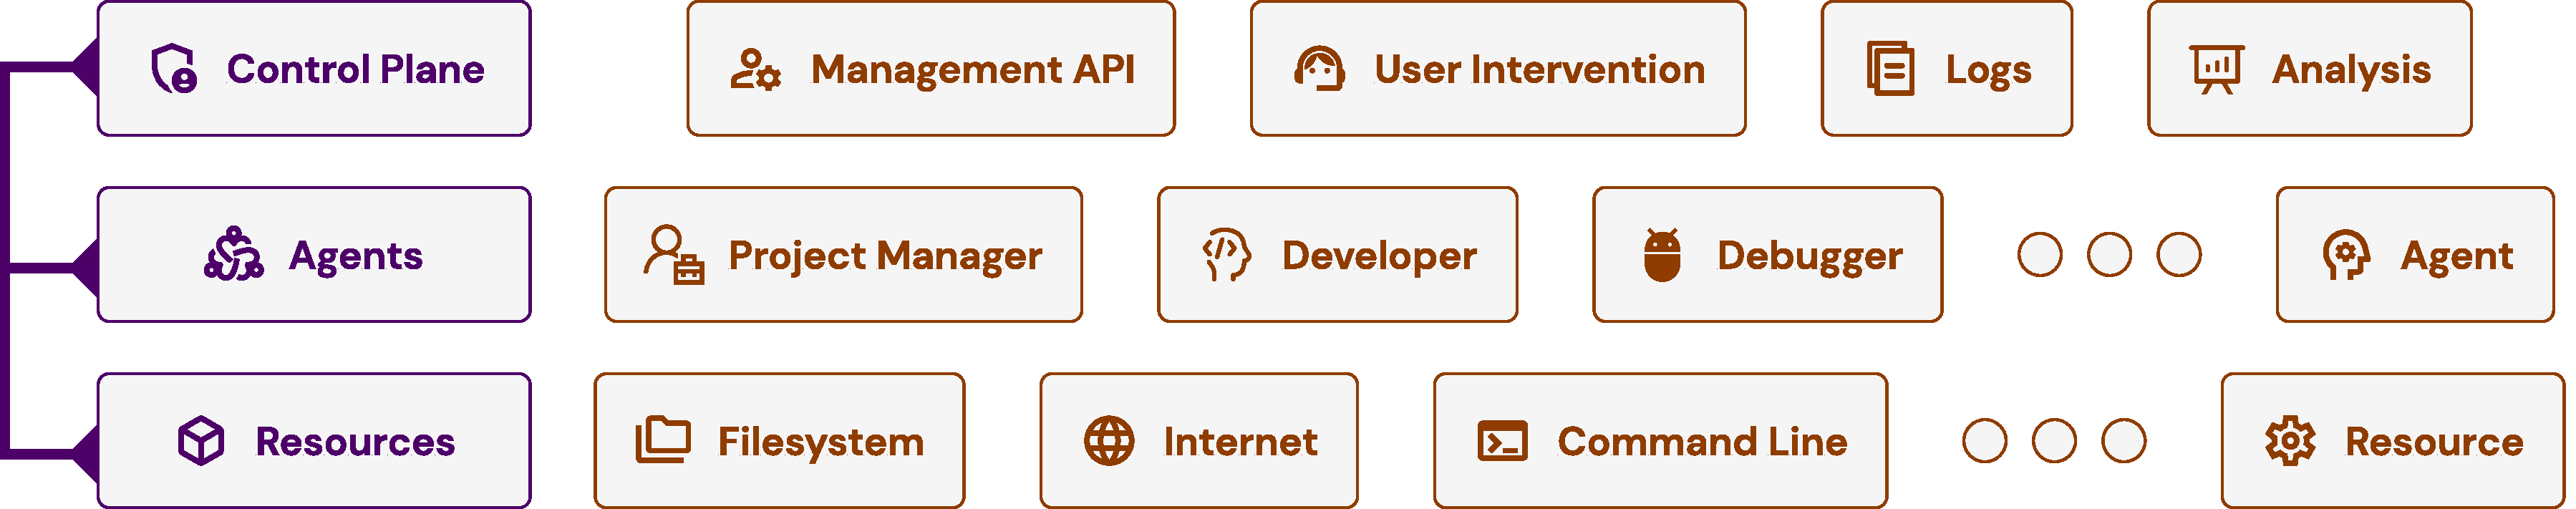
\includegraphics[width=\textwidth]{figures/components.pdf}
  \caption{The system comprises a control plane, a service mesh, and a resource layer. The \textbf{control plane} orchestrates agents and manages resources. The \textbf{agents} are responsible for doing the generation, acting on different resources. \textbf{Resources} provide an interface for agents to interact with their environment, such as the filesystem and the internet, to get context and complete tasks.}
  \label{fig:components}
\end{figure*}
As shown in Figure~\ref{fig:components}, the Solus system comprises three primary components:
\begin{enumerate}
  \item \textbf{Control Plane}: The control plane orchestrates agents and manages resources. It also provides an entry point for users to interact with the system and monitor operations. Agents and Resources beam all actions to the control plane, which analyzes them and decides how to proceed.
  \item \textbf{Agents}: Agents act on resources and interact with each other to complete the task given by the user. Agents are customizable components with roles and a set of allowed operations. They communicate with each other to regulate each other. For example, a Project Management agent may help a Software Engineer agent to stay working on items relevant to the business concerns of the system. Agents are also responsible for self-regulation and monitoring their resource usage.
  \item \textbf{Resources}: Agents interact with resources such as the filesystem, internet, and databases to complete tasks. Resources are abstracted away from agents, allowing us to optimize and shard them under the hood. Resources are also responsible for monitoring and reporting their usage to the control plane.
\end{enumerate}
The abstraction of agents and resources de-couples the generative process from the underlying infrastructure, allowing us to optimize and scale the system without affecting the generative process. It also provides room for expansion and customization, allowing us to create a plugin ecosystem for agent types and resource types.

\subsection{Inter-Service Communication}
\begin{figure}[t]
  \centering
  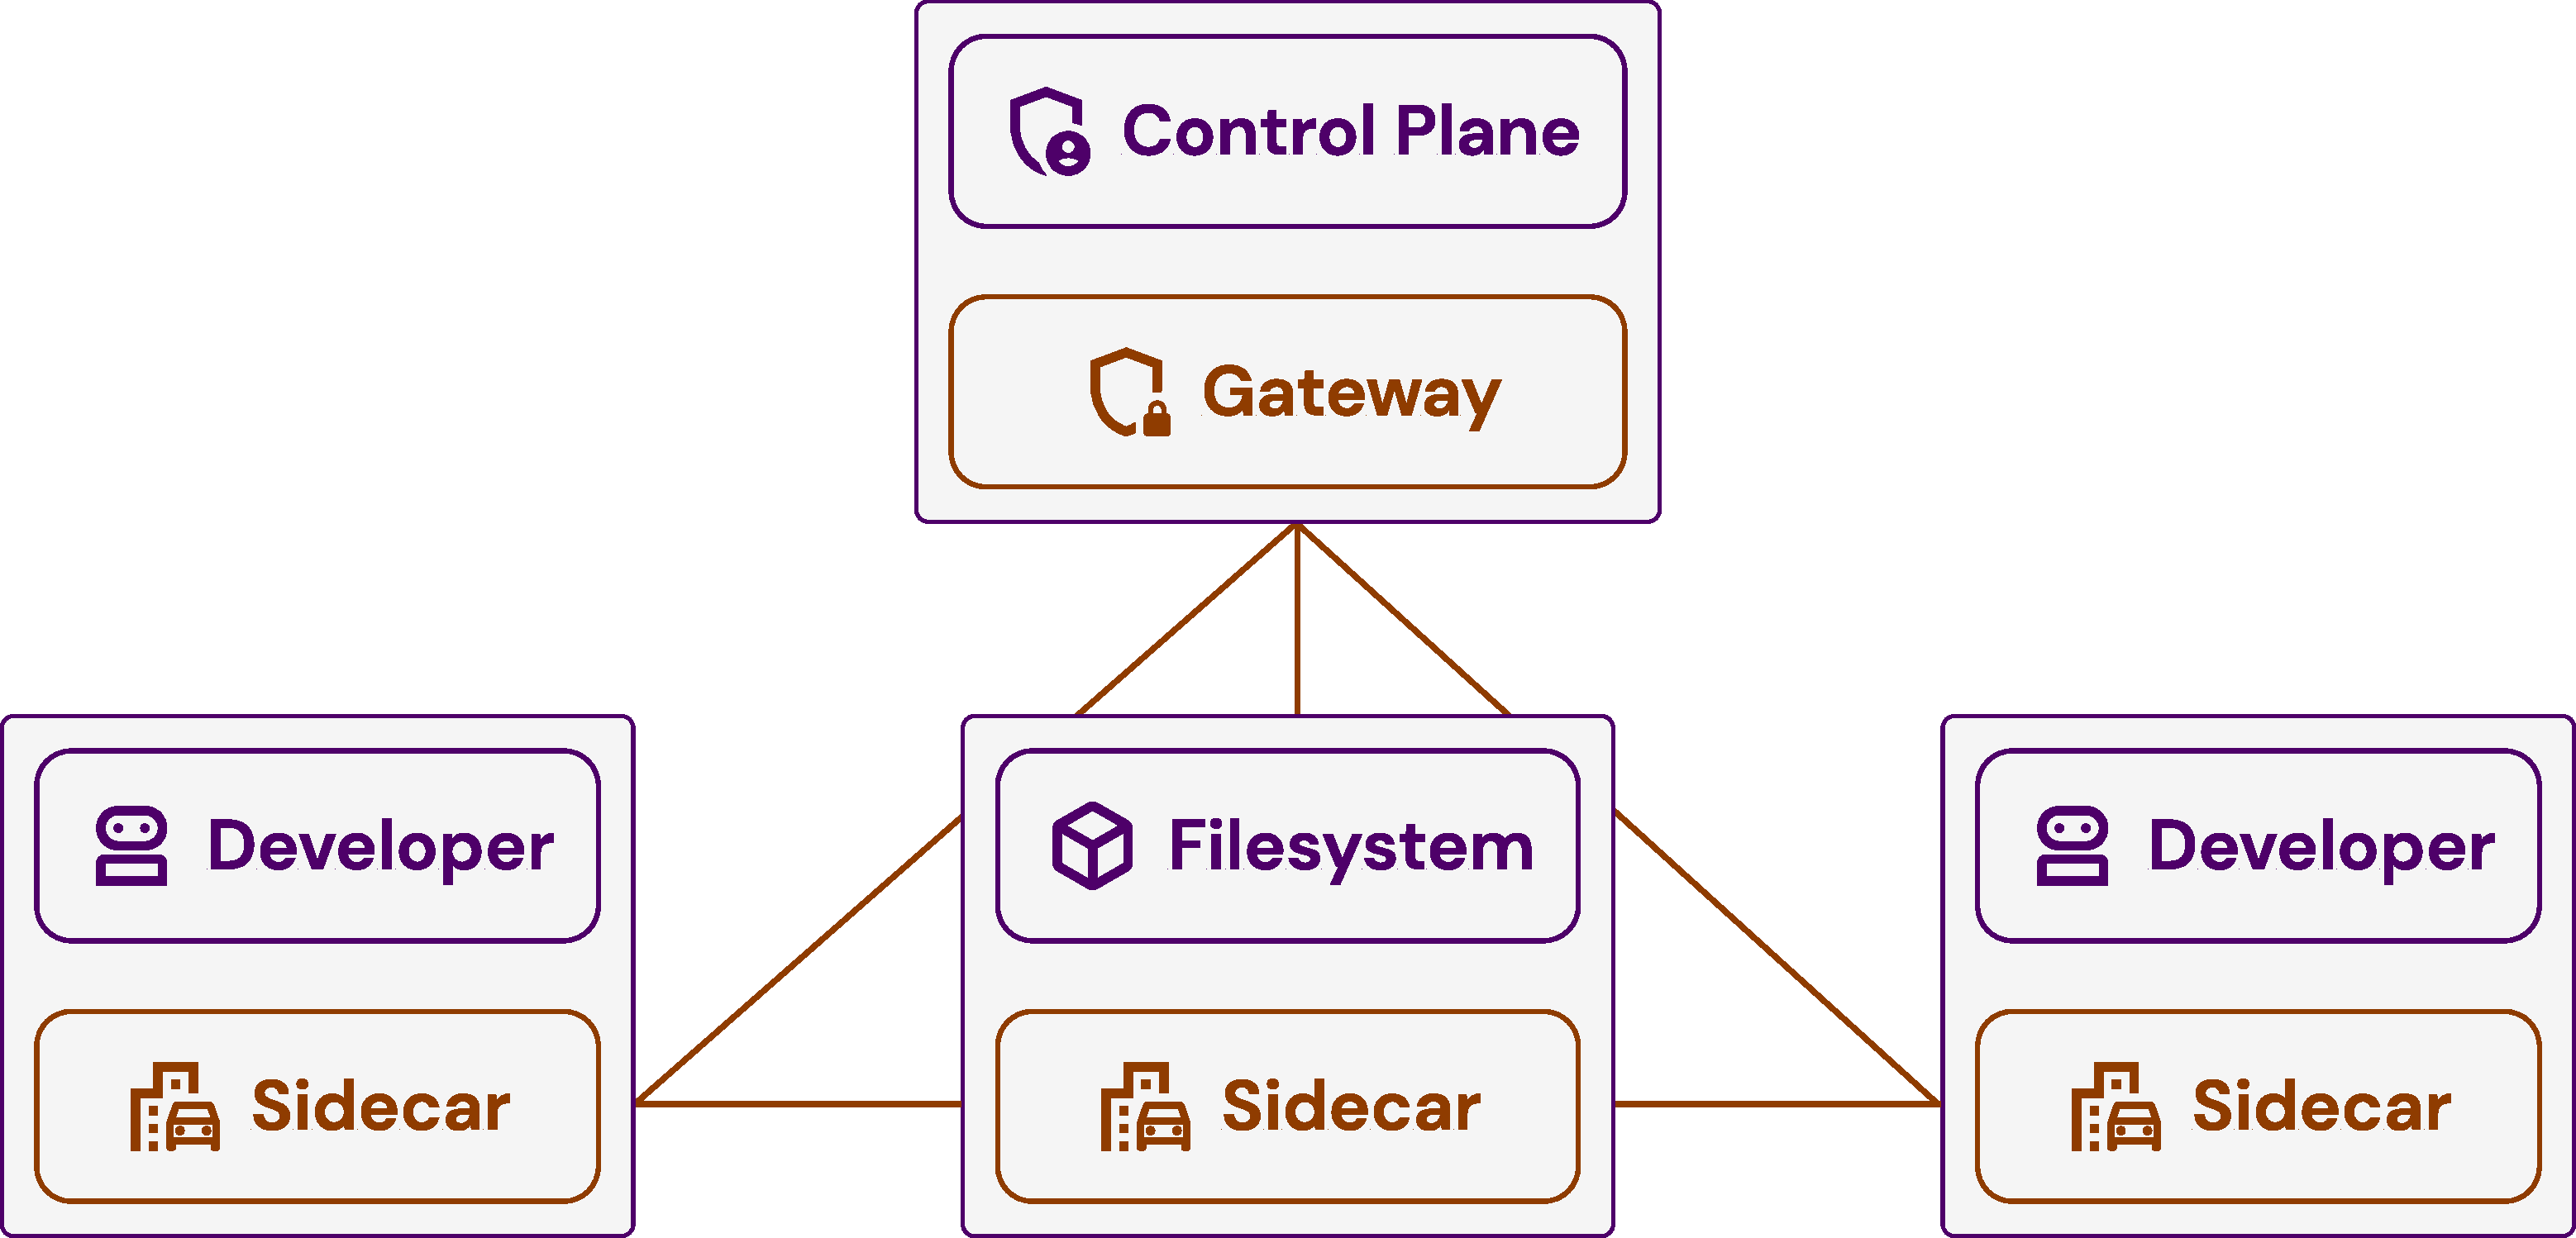
\includegraphics[width=\columnwidth]{figures/inter-service_interaction.pdf}
  \caption{The services interact through a service mesh. Sidecars intercept and standardize services' communications and beam them to the control plane.}
  \label{fig:inter-service_interaction}
\end{figure}
As shown in Figure~\ref{fig:inter-service_interaction}, the services interact through a service mesh. Sidecars intercept and standardize services' communications and beam them to the control plane. The control plane keeps logs of all system activity, intervening when needed or requested by the user. The other components of the system regulate their communications and complete actions independently. A service mesh allows agents and resources to handle their interactions while keeping a centralized log of all activity in the control plane. It will enable us to monitor and regulate the system while abstracting away the underlying infrastructure from the agents.

The service mesh design pattern was initially used to manage microservices in a cloud-native environment due to its de-coupling of the network layer from the application layer\cite{LiService}. Due to the scale and compute requirements of competent language models\cite{Touvron2023LLaMA}, we must run agents on separate machines. A service mesh allows us to scale the system horizontally without affecting the generative process.

\subsection{Agents}
\begin{figure*}[t]
  \centering
  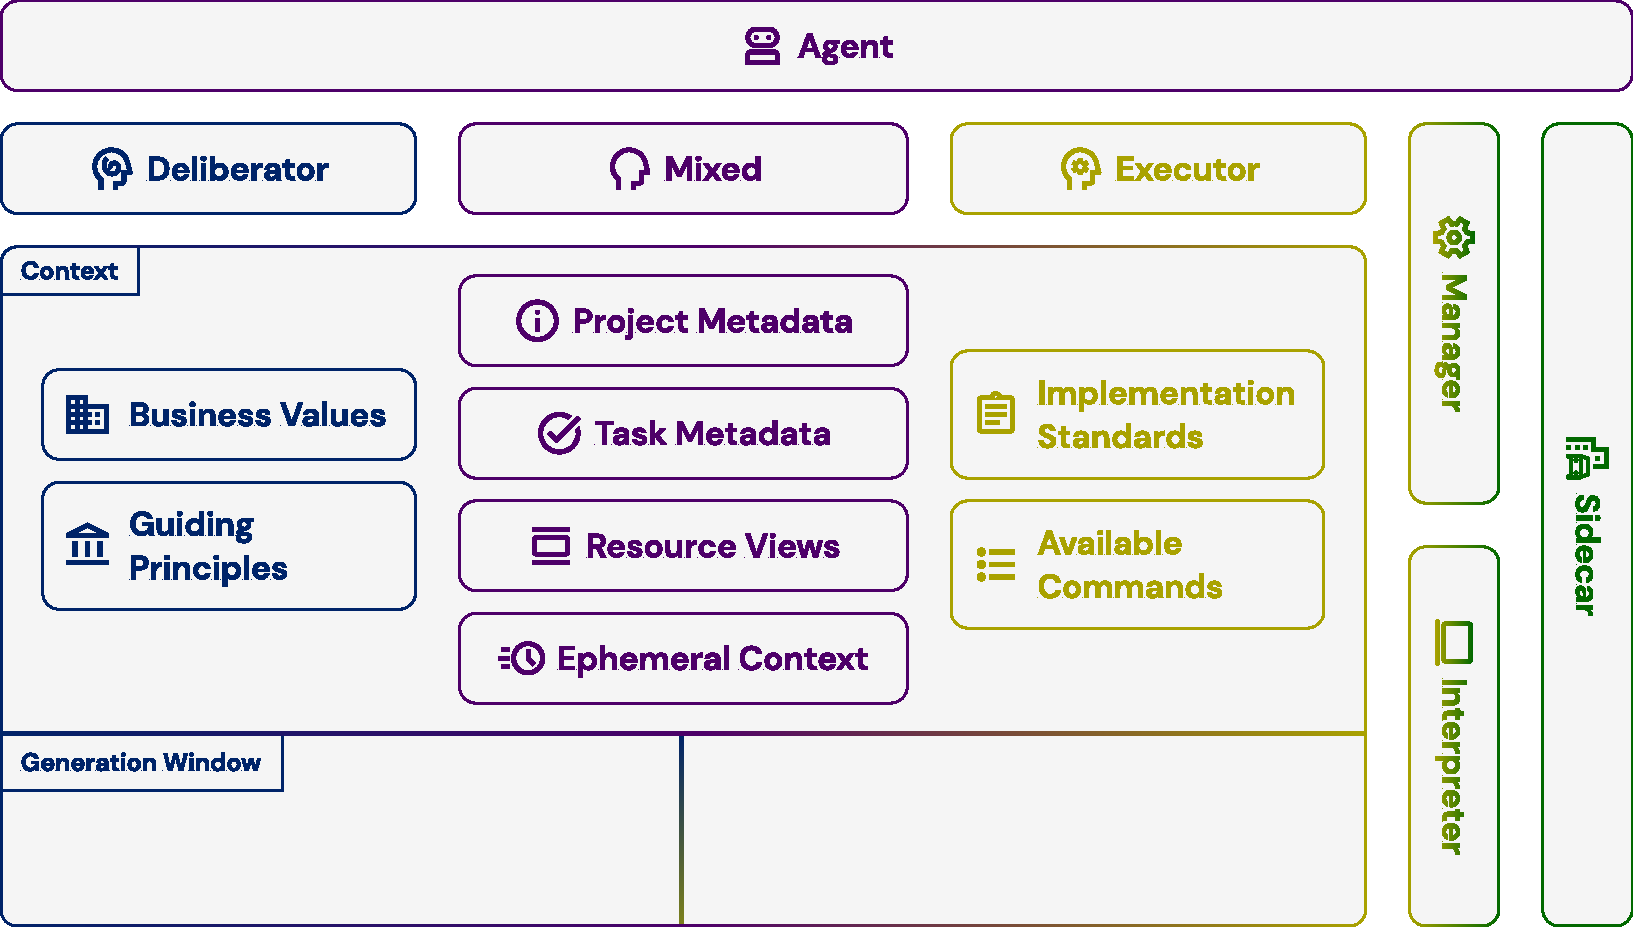
\includegraphics[width=\textwidth]{figures/agent.pdf}
  \caption{Agents represent the people in a software team. They act on resources and interact with each other to complete the task given by the user. They use two language models, a deliberator and an executor. The \textbf{deliberator} conducts unstructured reasoning about the current task, forming a critical chain of thinking and action. The \textbf{executor} takes the reasoning from the deliberator and converts it to commands according to a structured specification provided by the Agent's context. The \textbf{interpreter} serializes and parses the output from the executor, forming a set of requests to send to the manager. The \textbf{manager} manages the lifecycle of the agent's generations and updates the local context. It takes commands from the interpreter to send through the sidecar. As described in Figure~\ref{fig:inter-service_interaction}, the \textbf{sidecar} manages all inbound and outbound requests between agents, beaming them to the control plane for processing and delegating them to the manager.}
  \label{fig:agent}
\end{figure*}
As shown in Figure~\ref{fig:agent}, agents represent the people in a team, interacting with resources and each other to complete the project tasks. We utilize two models, a deliberator and an executor, to collaborate on tasks. Using a model to reason throughout a task before performing actions improves the quality of generations\cite{Fu2023Improving}, similar to how humans reason through ideas before acting on them (most of the time). The deliberator gets high-level context, such as business values and principles. The executor gets lower-level context like implementation standards-for example, a codebase style guide-and its available commands. The models also have shared context about the project, current task, resource views, and ephemeral context (short-term memory).

Resource views are the agent's view of the resources it interacts with. For example, a software engineer agent may have a view of the codebase, the filesystem, and the internet. A human software engineer opens files in their editor and websites in their browser and uses the terminal to run commands. The agent's resource views are similar to the human's but are abstracted away from the agent. The agent does not know how to open a file or run a command. It only knows how to request the manager to open a file or run a command. The manager then delegates the request to the sidecar, updating the resource view when the action is complete.

Their ephemeral context includes a shared truncated history of the deliberator and executor's generations. This context simulates the short-term memory human developers use when executing tasks.

\subsection{Resources}
\begin{figure}[t]
  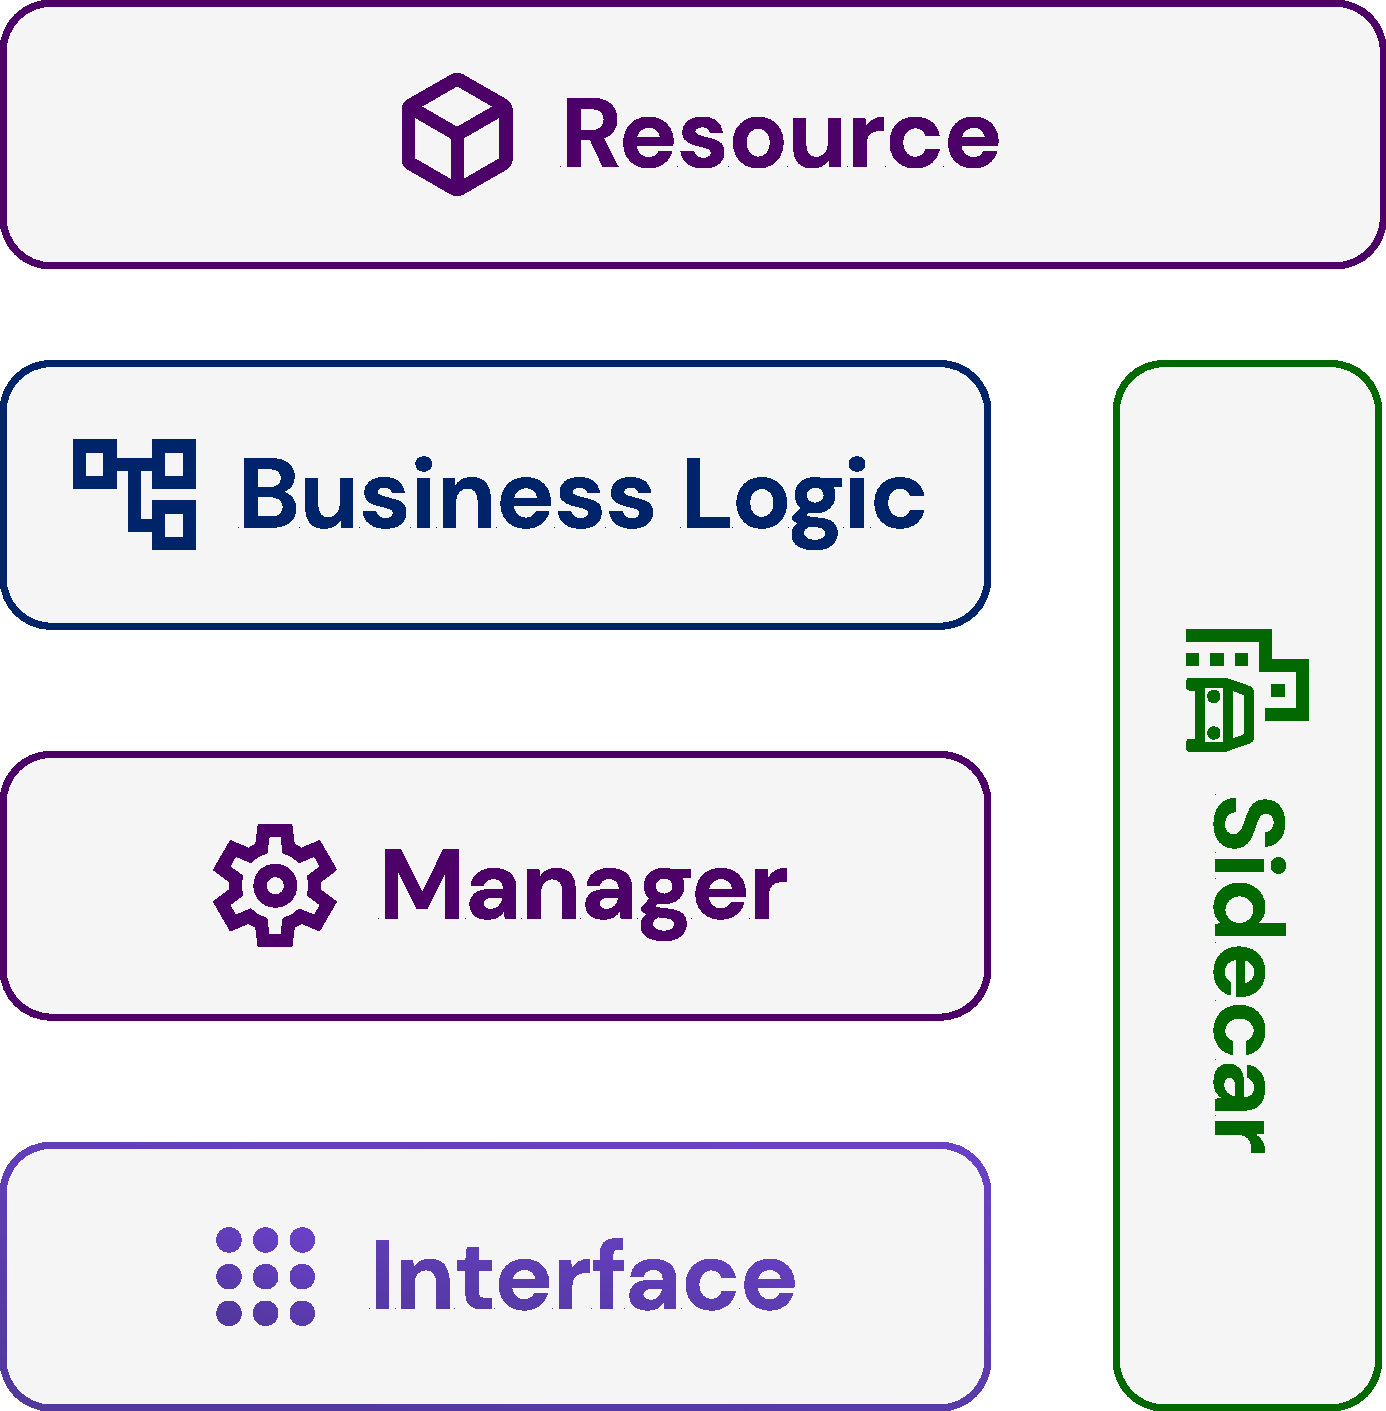
\includegraphics[width=\columnwidth]{figures/resource.pdf}
  \caption{Resources manage all the underlying infrastructure and outside entities in the generation process. They consist of \textbf{business logic} that accesses the resource itself, a \textbf{manager} that schedules actions and monitors the resource, an \textbf{interface} that contains and validates the specification for interacting with the given resource, and a \textbf{sidecar} that manages all inbound and outbound requests made to the resource, beaming to the control plane for processing and delegating them to the manager.}
  \label{fig:resources}
\end{figure}
As shown in Figure~\ref{fig:resources}, resources interact with all entities involved with the task to complete it. For example, a software engineer agent may need to interact with the filesystem, the internet, and a database to complete a task. The agent will send requests to the manager, such as to get the contents of a file or run a command. The manager will then delegate the request to the sidecar, returning the result to the agent once the action is complete.

The resources are abstracted from the agents, allowing us to implement effective access control and rate limiting. For example, a software engineer agent may access the filesystem and the internet, not the database. If the software engineer agent is compromised, the attacker cannot access the database due to the access control implemented in the database resource. The resource also allows us to implement rate limiting, preventing the agent from overloading expensive resources. For example, the agent may only be able to run one command at a time, preventing it from overloading the CPU.
\bibliography{whitepaper}
\end{document}